\chapter{Theoretical Background and Tools}
\label{chapter:Background}
This chapter describes algorithms and tools used in this project. It does not go into the details of each algorithm but it contains sufficient information to understand all the tools that we leveraged in interactive segmentation and recognition.
\section{Used Algorithms}
\subsection{RANSAC}
In order to explain the 3D features that were used as trackable parts of the point cloud in interactive segmentation for textuless objects basic understanding of RANSAC algorithm is needed. RANSAC stands for RAndom SAmple Consensus and it is an iterative algorithm that enables to find parameters of a mathematical model in the set of data containing outliers. The pseudocode of the algorithm is presented in Alg. \ref{alg:ransac}. 

\begin{algorithm}[htb!]
\While {$iterations < k$}
{
$maybe\_inliers$ := n randomly selected values from data
$maybe\_model$ := model parameters fitted to $maybe\_inliers$
$consensus\_set$ := $maybe\_inliers$

\ForEach {point in data not in $maybe\_inliers$}
{

\If {point fits $maybe\_model$ with an error $< t$}
{
add point to $consensus\_set$
}

}

\If {number of elements in $consensus\_set > d$}
{
(this implies that we may have found a good model,now test how good it is)\\
$this\_model$ := model parameters fitted to all points in $consensus\_set$\\
$this\_error$ := a measure of how well $this\_model$ fits these points\\



\If {$this\_error < best\_error$}
{            (we have found a model which is better than any of the previous ones,
            keep it until a better one is found)\\
            $best\_model$ := $this\_model$\\
            $best\_consensus\_set$ := $consensus\_set$\\
            $best\_error$ := $this\_error$\\
}


}
    increment iterations

}


\caption{RANSAC algorithm.}
  \label{alg:ransac}
\end{algorithm}

The most common example to explain RANSAC is a line fitting task in the 2D point dataset that contains outliers as shown in Fig. \ref{fig:ransac}. In the given dataset the algorithm would randomly pick two points and create a line equation that contains both of them. In the next step number of inliers is counted. Inliers meaning all the points that are lying within a certain threshold away from the line. If the number of inliers is bigger that the biggest number of inliers so far then it is saved. There are different implementation of RANSAC where the algorithm can run as long as there is not enough number of inliers or as the difference between them is becoming relatively small. As the result one obtains the best match to the given model that was found.

It is worth noticing that RANSAC algorithm can be used with many different models. In case of our system we use RANSAC to find the best fit to a line, a corner, a cylinder and a circle models. 



\begin{figure}
%\centering

{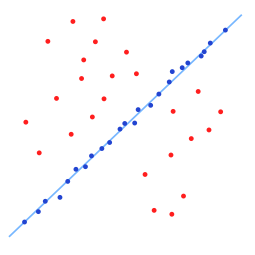
\includegraphics[width=0.5\columnwidth]{figures/ransac.png}}

\caption{RANSAC line fitting algorithm on an illustrative dataset.}
\label{fig:ransac}
\end{figure}



\subsection{3D and 2D Features}
As mentioned in the previous section RANSAC algorithm is the main tool used to extract 3D features on the objects. The differences between different geometric features that we are using is in the models used in RANSAC. We use a different mathematical representation of a feature, for example, a line or a cylinder, in order to extract it from the point cloud. 3D features are used only in the interactive segmentation of textureless objects part of the system. Our object recognition system employs various detectors and descriptors in the image space to extract and match 2D features.

In order to understand different 2D features that were used in our system it is crucial to be familiar with the concepts behind detectors, descriptors and matchers. We, as humans, have no problems in detecting distinctive features in the images we see. Moreover we can easily realize that there are some features in the image that we have seen before. To reproduce this process for an autonomous system there are multiple components needed since an image is seen by a computer as a simple set of pixel values without any high level meaning. First, the system has to detect points of interest in the image that are distinctive enough to find the same points multiple times. The algorithms that are behind this process are called detectors and their goal is to simply find good features. Having the region detected the next step is to describe the found features such that there is a big chance to find the same features later on under different conditions. The task of describing the found points belongs to a detector. In the next subsections we will describe different detector-descriptor pairs that were used in the object recognition part of the thesis.

\subsubsection{SIFT}
SIFT~\cite{lowe2004distinctive} stands for Scale Invariant Feature Transform and is one of the most popular descriptor-detector pair. The SIFT features are invariant to scale and rotation as well as invariant to some extend to illumination changes and the viewpoint of the camera.  

The detector is employed in different scales and the algorithm is looking for the highest response in difference of Gaussian which corresponds to the the best scale where the feature was found. In order to detect the local maxima and minima of difference of Gaussian function, the point of interest is compared to its eight neighbors in the current scale and to the respective pixels in the scale one level above and below. As the next step D.Lowe employs filters that remove low contrast and edge responses using Hessian Matrix on difference of Gaussian. After all these steps the found points are considered as being robust enough to be further used.

Once the feature is found, it is crucial to use the feature descriptor to describe it in an distinctive manner.  SIFT detector solves rotational invariance problem by calculating orientations of the feature neighboring pixels and creating histogram of them. After smoothing operations the the peak of smoothed histogram is assigned as the general orientation of the SIFT feature. Moreover, the feature is afterwards rotated such that it can be matched against a similar feature even if they have different orientations in the original image. Thus, the rotational invariance is considered as one of the properties of SIFT.

\begin{figure}
%\centering

{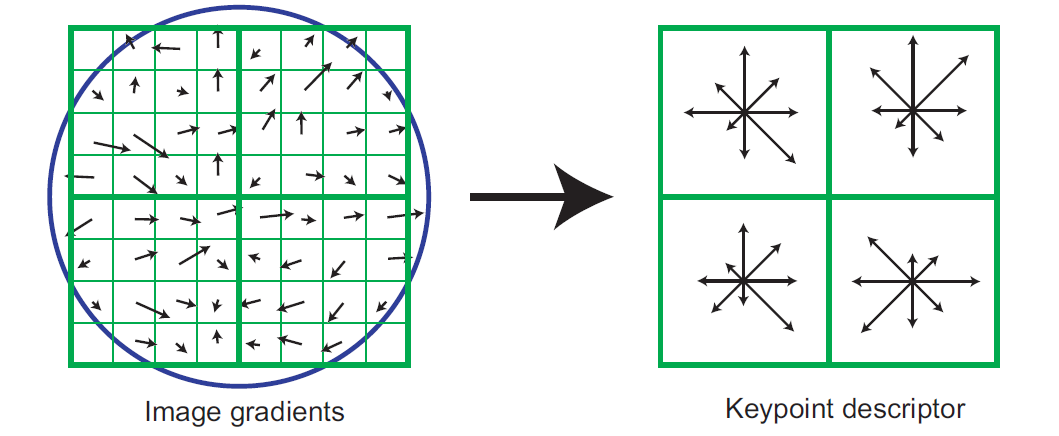
\includegraphics[width=1\columnwidth]{figures/sift.png}}

\caption{SIFT descriptor. Source:~\cite{lowe2004distinctive}}
\label{fig:sift}
\end{figure}

In order to make SIFT invariant to remaining variations - illumination and 3D viewpoint a descriptor of keypoint is created. As shown in Fig. ~\ref{fig:sift} the orientation histogram in 8 directions is computed. The process is based on image gradients and regards every pixel surrounding the keypoint. This representation shows a feature that also contains information about its surroundings which makes it more distinctive under different conditions.

\subsubsection{FAST and FREAK/BRIEF}
We are not sure if we will be using these features so let's see first.



\subsection{Point Cloud Processing}
In this section we would like to describe some of the algorithms that we used to process the point clouds received from the Kinect sensor. The definition of the point cloud is provided by R. Rusu in~\cite{Rusu_ICRA2011_PCL} and states the following:

A point cloud is a data structure that provides a representation of the 3D data visible by the depth sensor. This data structure consists of 3D points that have X, Y and Z component and are sampled from the underlying surface.  

Since the received point clouds are not perfect and need some pre-processing we take extensive use of the open source Point Cloud Library (PCL). Algorithms that were especially used in our work are described in the following sections.

\subsubsection{Voxel Grid Filtering}
It is a very common practice to reduce the number of points in the point cloud before further proceedings. The reason for that is that the process becomes faster and one does not require a lot of memory space to store the data. One of the methods to downsample a point cloud is voxelized grid approach.

A 3D voxel grid is a set of cubes that surround the points in the point cloud. Each of them contains a certain number of points which can be approximately represented by their centroid or the center of the cube. By approximating the points in the cube with one point we decrease number of points in the point cloud significantly. 

\subsubsection{Plane Removal}
Plane removal algorithm is one of the most popular pre-processing steps in perception algorithms. Using RANSAC algorithm with the model of a plane it is possible to select the biggest plane from the current point cloud. Having the indices of the points that form the biggest plane in the point cloud, it is possible to extract the plane itself and eventually, remove it. 

This process simplifies the further work on the point cloud. For example, having done this step, it is possible to segment the objects based on the euclidean clustering algorithm described in the section below.


\subsubsection{Euclidean Clustering}
The objective of the Euclidean Clustering algorithm is to group points into multiple clusters based on the euclidean distance between neighboring points. The algorithm takes each point and checks if there exist any neighboring points within certain euclidean distance from this point. If so, then these points are added to the same cluster and the procedure continues for each of them. If the found point was already examined then it is not taken into consideration again. If all the points within the set distance were proceeded the cluster is considered as finished and algorithm continues with another set of points. The algorithm runs as long as all the points are clustered. 

Euclidean Clustering algorithm enables simple segmentation of objects in uncluttered scene which can be further used in many applications.   

\subsection{Particle Filter}
In statistics, a particle filter, also known as a sequential Monte Carlo method (SMC), is a sophisticated model estimation technique based on simulation.[1] Particle filters are usually used to estimate Bayesian models in which the latent variables are connected in a Markov chain — similar to a hidden Markov model (HMM), but typically where the state space of the latent variables is continuous rather than discrete, and not sufficiently restricted to make exact inference tractable (as, for example, in a linear dynamical system, where the state space of the latent variables is restricted to Gaussian distributions and hence exact inference can be done efficiently using a Kalman filter). In the context of HMMs and related models, "filtering" refers to determining the distribution of a latent variable at a specific time, given all observations up to that time; particle filters are so named because they allow for approximate "filtering" (in the sense just given) using a set of "particles" (differently weighted samples of the distribution).

Particle filters are the sequential (online) analogue of Markov chain Monte Carlo (MCMC) batch methods and are often similar to importance sampling methods. Well-designed particle filters can often be much faster than MCMC. They are often an alternative to the Extended Kalman filter (EKF) or unscented Kalman filter (UKF) with the advantage that, with sufficient samples, they approach the Bayesian optimal estimate, so they can be made more accurate than either the EKF or UKF. However, when the simulated sample is not sufficiently large, they might suffer from sample impoverishment. The approaches can also be combined by using a version of the Kalman filter as a proposal distribution for the particle filter.[citation needed]


\section{Used Tools}
\subsection{Kinect}

\begin{figure}
%\centering

{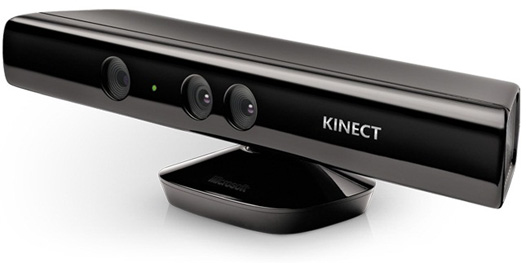
\includegraphics[width=0.5\columnwidth]{figures/kinect.jpg}}

\caption{The Kinect sensor. Source: http://www.engadget.com}
\label{fig:kinect}
\end{figure}

Kinect (codenamed in development as Project Natal) is a motion sensing input device by Microsoft for the Xbox 360 video game console and Windows PCs. Based around a webcam-style add-on peripheral for the Xbox 360 console, it enables users to control and interact with the Xbox 360 without the need to touch a game controller, through a natural user interface using gestures and spoken commands.[9]

The depth sensor consists of an infrared laser projector combined with a monochrome CMOS sensor, which captures video data in 3D under any ambient light conditions.[9][34] The sensing range of the depth sensor is adjustable, and the Kinect software is capable of automatically calibrating the sensor based on gameplay and the player's physical environment, accommodating for the presence of furniture or other obstacles.[35]
\subsection{PR2}

\begin{figure}
%\centering

{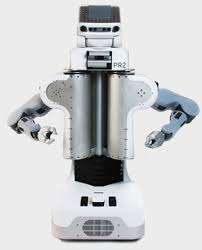
\includegraphics[width=0.5\columnwidth]{figures/pr2.jpeg}}

\caption{PR2 robot. Source: http://www.willowgarage.com}
\label{fig:pr2}
\end{figure}

The PR2 stands for 'personal robot' and it is a humanoid robotics platform created by Willow Garage - a robotics company based in Menlo Park, CA. The platform has two arms and grippers and an omnidirectional base as shown in Fig. \ref{fig:pr2}. Additionally, it contains multiple sensors including Kinect and tactile sensors. 8-core servers provide the robot's computing power and a 2TB hard drive serves as the robot's memory.  

In our system we used the PR2 as the main robotics platform. We took use of robot's sensors as well as actuator by implementing the manipulation strategies on the robot.

\subsection{ROS}
Robot Operating System (ROS) is a framework designed as an equivalent of an operating system but for robotics applications. 

There are two main components of ROS: a) standard operating system-like core functions and b) ros packages that can be created by the open source community. The former component contains various services such as messaging processes or package management whereas the latter one is designed for users to contribute and share their applications. ROS is known for containing multiple robotics applications such as motion planning, perception or control.

Our system uses ROS-infrastructure heavily by exploiting its communication system that enables us to communicate synchronously as well as asynchronously between different elements of the code. The whole system is wrapped into multiple ROS packages and is shared with ROS open source community.




\subsection{Gazebo}
Gazebo is an open source physics simulator that can simulate multiple robots, their sensors, actuators and third party objects. It is also integrated into ROS infrastructure which makes it easier to simulate the real robot's behaviour, including readings from the sensor or motor control. 

In our system Gazebo was used to verify the push point hypothesis with the PR2 robot. It enabled us to test multiple scenarios in very short time without using an actual robot.


\subsection{PCL}
The Point Cloud Library (PCL) is an open source C++ library that contains tools for point cloud processing. It consists of many algorithms that enable to filter the data, extract features, reconstruct surface, register multiple point clouds and object segmentation, among others. The architecture of the library follows object-oriented design patterns hence it is modular and easy to use. PCL work on multiple platforms including Linux, MacOS, Windows and Android. 

Throughout our project PCL was the most frequently used library as enabled us to implement state-of-the-art 3D processing algorithms very fast and efficiently.  

\subsection{OpenCV}
OpenCV is an Open Source Computer Vision library that contains over 2500 optimized algorithms in Computer Vision. It was used very extensively throughout our system. It is also one of the most popular open source software with 7 million downloads by far. It consists of multiple interfaces such as C++, C and Python that supports all the major platforms. The architecture of the library is rather flat meaning that it contains mainly function calls that highly object oriented design which is much different in comparison to PCL.

Many algorithms from our system including SIFT implementation and image morphology operations were taken from OpenCV Library. 








